 \documentclass{report}
\usepackage[utf8]{inputenc}    
\usepackage[T1]{fontenc}
\usepackage[francais]{babel}
\usepackage{wrapfig}
\usepackage{graphicx}
\usepackage{listings,xcolor}
\usepackage{appendix}
\usepackage{adjustbox}
\usepackage{titling}

%Géométrie des pages
\usepackage{geometry}
\geometry{hmargin=2.5cm,vmargin=2.5cm}

%Définition des couleurs pour le code xml
\definecolor{colorxmlnode}{rgb}{0.2, 0.2, 0.2} 
\definecolor{maroon}{RGB}{178 34 34}


%Profondeur des compteurs et de la tableofcontents
\setcounter{secnumdepth}{3}
\setcounter{tocdepth}{2}


%lst xml
\lstdefinelanguage{XML}
{
  basicstyle=\ttfamily,
  morestring=[s]{"}{"},
  morecomment=[s]{?}{?},
  morecomment=[s]{!--}{--},
  commentstyle=\color{darkgreen},
  moredelim=[s][\color{black}]{>}{<},
  moredelim=[s][\color{red}]{\ }{=},
  stringstyle=\color{blue},
  identifierstyle=\color{maroon}
}


\addto\captionsfrench{%
  \renewcommand\appendixname{Annexe}
  \renewcommand\appendixpagename{Annexes}
}

%Définition des commandes \noeud et \classe
\newcommand\classe[1]{\mbox{\textit{#1}}}
\newcommand\noeud[1]{\textcolor{colorxmlnode}{<\mbox{#1}>}}


\setlength{\droptitle}{-10em}   % This is your set screw


\pretitle{%
  \begin{center}
  \LARGE
  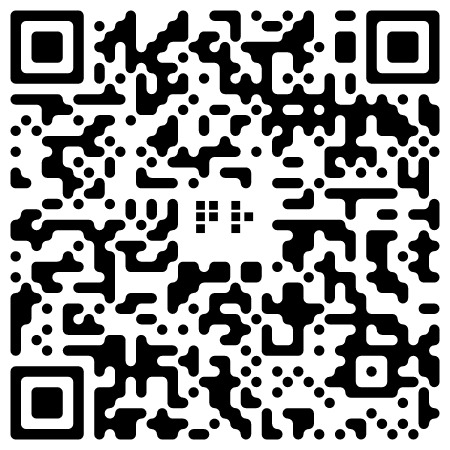
\includegraphics[width=5cm,height=5cm]{img/qr.jpeg}\\[30px]
}
\posttitle{\end{center}}


\title{% 
		Développement d'un couple d'applications bureau et mobile\\ \large
		Génération et lecture de QR Codes pour l'institut Montéclair}
\author{David \bsc{Dembele}\\ Alassane \bsc{Diop}\\
		Jules \bsc{Leguy}\\ Rahmatouwalet \bsc{Mohamedoun}}
\date{Décembre 2017}



\begin{document}

\maketitle

\tableofcontents

\chapter{Introduction}

	\section{Contexte}
		
\par
Dans le cadre du module Concrétisation Disciplinaire de notre première année de Master 1 mention Informatique à l'Université d'Angers, nous avons développé une application de bureau et poursuivi le développement d'une application mobile.

\par
Ces applications répondent à une demande de l'Institut Montéclair à Angers, dans le but d'apporter une dimension ludique à l'enseignement pour les mal-voyants et non-voyants inscrits à l'institut.

\par
Ce projet a été encadré par Corentin \bsc{Talarmain} et Thomas \bsc{Calatayud}, deux étudiants en deuxième année de Master, dans le cadre de leur module Gestion de Projet.\\

\par
L'objectif du projet est de fournir la possibilité aux transcripteurs de l'institut un moyen de générer des QR Codes contenant du texte et des sons et pouvant être interprétés par une application mobile. Une première version de l'application mobile avait déjà été développée par Corentin \bsc{Talarmain} lors de son TER\footnote{Travail Encadré de Recherche} de fin de première année de Master. Celle-ci fournissait déjà la possibilité de lire avec une voix de synthèse du texte contenu dans des QR Codes.
Nous avons donc développé une application de bureau permettant de générer ces QR Codes selon les contraintes décrites dans le cahier des charges. Nous avons également adapté l'application mobile existante à notre nouveau format de données.

	
	\section{Objectifs}
		\par
Les transcripteurs souhaitaient néanmoins étendre les fonctionnalités de l'application mobile initiale, qui présentait quelques inconvénients limitant son utilisation. Ne présentant que la possibilité de lire des QR Codes, elle imposait le passage par des sites internet pour en générer. On ne pouvait ainsi pas contrôler la taille maximale des QR Codes générés, parmi lesquels certains étaient trop gros pour être détectables par l'application. En outre, elle ne fournissait pas la possibilité de lire des sons à partir de données contenues dans un QR Code.\\

\par
Les transcripteurs de l'institut nous ont également fourni deux demandes précises autour desquelles nous avons structuré notre projet. La première demande était de pouvoir utiliser les QR Codes comme légendes de cartes de géographie pour des lycéens. Cela implique de pouvoir gérer la lecture de QR Codes adjacents dans un ordre prédéfini, peu importe l'ordre de lecture effectif (LIEN FAMILLES).
\par
L'autre demande était de pouvoir utiliser des QR Codes pour lire des sons dans les pages d'un livre pour enfants, sans avoir nécessairement accès à internet au moment de la lecture. Pour cela, un ou plusieurs QR Codes sur la page de couverture doivent permettre le téléchargement de tous les sons contenus dans le livre (LIEN ENSEMBLE).
\par
En outre, un espace central contenant du texte en braille devait pouvoir être inséré au centre des QR Codes, pour permettre aux non-voyants de les localiser (LIEN GENERATION QR).


		
\chapter{Modélisation}

	\section{Types de QRCodes}
		\par
À partir des contraintes définies dans les cahier des charges (voir \ref{objectifs}), il a fallu définir précisément quels types de QR Codes allaient être crées. Une première version de notre architecture collait aux besoins de l'Institut Montéclair qui nous ont été transmis. Elle comprenait des QR Codes pour les cartes géographiques, des QR Codes pour les pages d'un livre et des QR Codes pour les pages de couverture des livres. Mais cette architecture s'est avérée trop spécifique et empêchait les transcripteurs de l'institut de créer des QR Codes pour d'autres supports.\\

\par
Nous avons donc créé une seconde version qui respectait les contraintes transmises par l'institut tout en étant la plus généraliste possible, afin d'être utilisable dans tous les contextes compatibles avec les contraintes transmises. Cette architecture est composée de QR Codes contenant un ensemble de textes et de fichiers et pouvant être organisés en familles afin d'être lus dans un ordre prédéfini (les QR Codes atomiques), et de QR Codes contenant un ensemble de liens vers des sons devant être téléchargés sans être joués (les QR Codes ensembles).
		
	\section{Représentation des données}
		\par
Les QR Codes devant stocker plus d'informations que dans la version initiale de l'application mobile, il nous a fallu définir une structure de données pour les représenter. Cette représentation s'est construite parallèlement à l'élaboration des types de QR Codes (voir \ref{typesQR}) et à celle du Modèle (voir \ref{architecture}), afin d'assurer la cohérence de l'ensemble.\\

\par
Dans le but de minimiser la quantité d'informations contenue dans le QR Code, nous nous sommes appuyés sur un modèle séparant les données nécessaires à la lecture par l'application mobile et les données nécessaires seulement au chargement à l'identique du QR Code après son enregistrement par l'application de bureau.\\

\par
Pour comprendre, prenons l'exemple d'une page d'un livre pour enfant décrivant des animaux. Afin de rendre cette page plus ludique pour les non-voyants, les transcripteurs de l'institut souhaiteraient coller sur cette page un QR Code pour chaque animal décrit. Ces QR Codes contiendraient chacun un petit texte explicatif et le cri de l'animal. Ils souhaiteraient qu'ils soient lus dans un ordre prédéfini, et qu'un texte en braille représentant les lettres \textit{QR} soit présent au centre de chacun des QR Codes. De plus, le QR Code devrait être bleu et le texte central en braille rouge afin qu'il puisse être imprimé en relief.

\par
Parmi ces données, certaines ne sont pas indispensables à l'application mobile pour interpréter le QR Code. Elle n'a par exemple pas besoin de connaître le texte en braille ou le nom du fichier contenant le cri de l'animal. Ces données seront en revanche nécessaires à l'application de bureau pour recharger les QR Codes à l'identique le jour où les transcripteurs voudront modifier la description de l'animal. Nous allons donc séparer ces données en deux parties : les données nécessaires à l'application mobile seront encodées dans le QR Code tandis que les données qui ne le sont pas seront insérées dans le fichier image, mais pas dans le QR Code en lui-même. Nous détaillons cette séparation dans le schéma suivant.



\begin{figure}[!h]
	\centering
   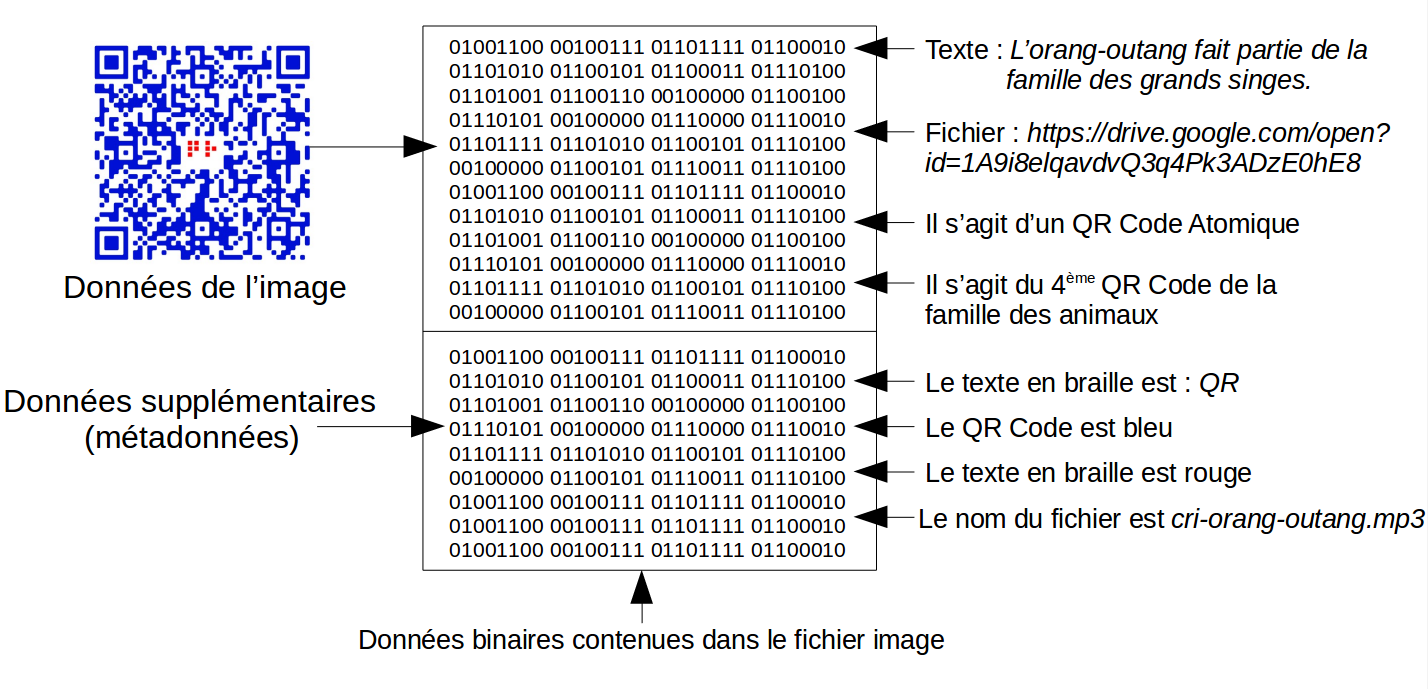
\includegraphics[scale=0.33]{img/schema_representation_donnees.png}
   \caption{Contenu d'une image d'un QR Code}
\end{figure}

\newpage
\par
Afin de stocker ces données de manière formelle, nous avons établi une structure de type XML\footnote{Extensible Markup Language} (voir \ref{compression}). Elle fait apparaître clairement la dichotomie entre les données stockées dans le QR Code (noeud \noeud{donneesUtilisateur}) et les données stockées dans les métadonnées de l'image (noeud \noeud{metadonnees}).
\par
Le type de QR Code (atomique ou ensemble) est indiqué par un attribut dans le noeud \noeud{donneesUtilisateur}. Ce noeud contient un noeud \noeud{contenu} contenant lui-même un ensemble de textes (\noeud{texte}) et de fichiers (\noeud{fichier}).
\par
L'appartenance à une famille (voir \ref{typesQR}) de QR Codes est indiquée par la présence d'un noeud \noeud{famille} ayant pour attributs le nom de la famille et la place du QR Code.
\par
La représentation formelle de l'exemple du QR Code orang-outang est visible dans la figure ci-dessous.

\begin{figure}[!h]
\begin{adjustbox}{minipage=\textwidth,bgcolor={RGB}{240 240 240}}

\lstset{language=XML}

\begin{lstlisting}
<qrcode>
  <donneesutilisateur type="atomique">
    <contenu>
      <texte>L'organg-outang fait partie de la famille 
             des grands singes.</texte>
      <fichier url="1A9i8elqavdvQ3q4Pk3ADzE0hE8"/>
    </contenu>
    <famille nom="animaux" ordre="4"/>
  </donneesutilisateur>
  <metadonnees>
    <fichiers>
      <fichier url="1A9i8elqavdvQ3q4Pk3ADzE0hE8" 
               nom="cri-orang-outang.mp3"/>
    </fichiers>
    <colorqrcode color="#1606e7"/>
    <textebraille texte="QR"/>
    <colorbraille color="#ea0000"/>
  </metadonnees>
</qrcode>
\end{lstlisting}

\end{adjustbox}
\caption{Représentation d'un QR Code}

\end{figure}\textbf{}
		

\chapter{Application de bureau}

	\section{Conception}
		
		\subsection{Langages}
			\par
Le choix des langages de programmation pour l'application de bureau a été discuté lors de la première séance. Nous avons évoqué le couple Java/Swing qui avait l'avantage d'être le plus simple à programmer et qui aurait été en cohérence avec l'application Android, mais qui nécessitait un environnement Java sur les machines des utilisateurs. Nous avons également évoqué le couple C++/Qt qui était le plus portable mais potentiellement trop lourd pour l'utilisation qu'on en aurait. 
\par
Les responsables du projet ont finalement opté pour le framework Electron entre les deux premières séances. Ce framework\footnote{Un framework désigne un ensemble cohérent de composants logiciels structurels, qui sert à créer les fondations ainsi que les grandes lignes de tout ou d’une partie d'un logiciel (Wikipédia).} permet de développer des applications de bureau avec des langages web (Javascript/HTML/CSS), et d'utiliser les modules Node.js. Ce choix a été motivé par l'intérêt qu'avait le Javascript d'être facilement utilisable pour accéder à Google Drive (REF STOCKAGE DRIVE).
			
		\subsection{Architecture}		
			\par
L'application est structurée selon un modèle MVC (Modèle Vue Contrôleur). Les données sont représentées par les classes du modèle, sont traitées par les classes du contrôleur et affichées par la vue. Nous utilisons en outre le patron de conception\footnote{Un patron de conception (souvent appelé design pattern) est un arrangement caractéristique de modules, reconnu comme bonne pratique en réponse à un problème de conception d'un logiciel. Il décrit une solution standard, utilisable dans la conception de différents logiciels. (Wikipédia)} Façade, qui nous permet de limiter la dépendance de la vue au contrôleur à une seule classe. Nous schématisons ces interactions dans la figure suivante.

\begin{figure}[!h]
	\centering
   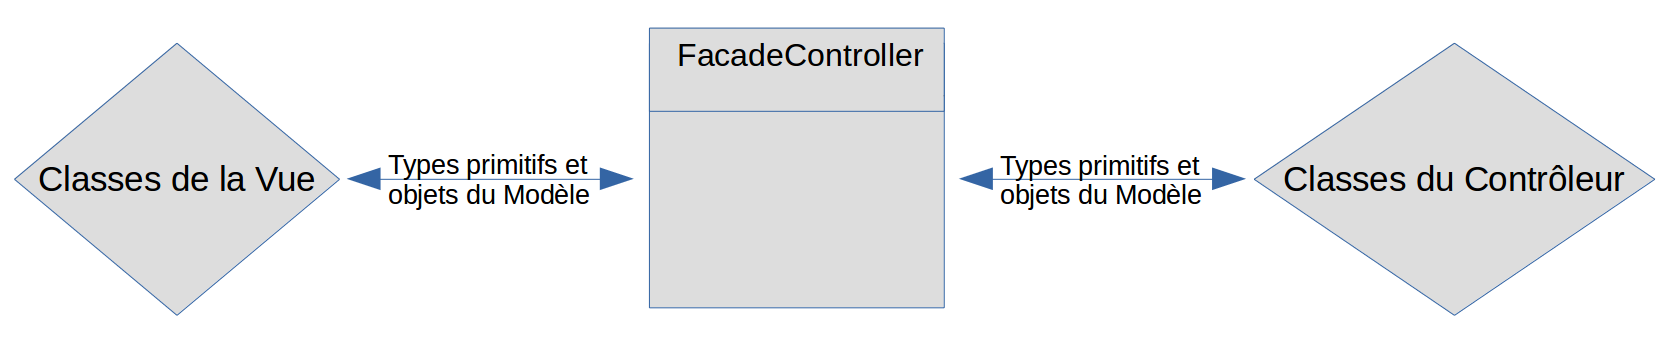
\includegraphics[scale=0.25]{img/facade.png}
   \caption{Interactions entre la vue et le contrôleur à travers la classe FacadeController}
\end{figure}

\par
Le modèle permet de représenter les QR Codes des différents types (voir \ref{typesQR}). Il est composé d'une superclasse abstraite \classe{QRCode}, étendue par deux classes \classe{QRCodeAtomique} et \classe{QRCodeEnsemble} représentant les spécificités des deux types de QR Codes gérés. Le modèle n'effectue pas de traitement des données mais fournit seulement des méthodes permettant d'y accéder et de les modifier, en faisant une abstraction de la façon dont elles sont représentées. Le diagramme UML des classes du modèle est visible ci-dessous.

\begin{figure}[!h]
	\centering
   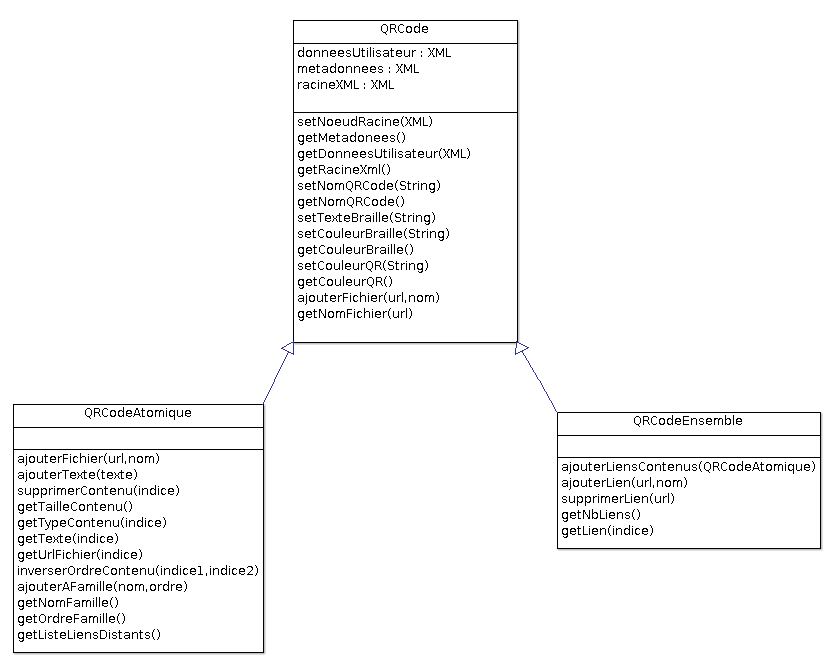
\includegraphics[scale=0.4]{img/modeleUML.png}
   \caption{Diagramme UML des classes du modèle}
\end{figure}

\par
Le contrôleur se charge de tous les traitements permettant de générer des images de QR Codes (voir \ref{generation}), ou d'instancier des objets du modèle à partir d'une image déjà générée (voir \ref{chargement}). L'architecture des classes du contrôleur est visible ci-dessous.


\begin{figure}[!h]
	\centering
   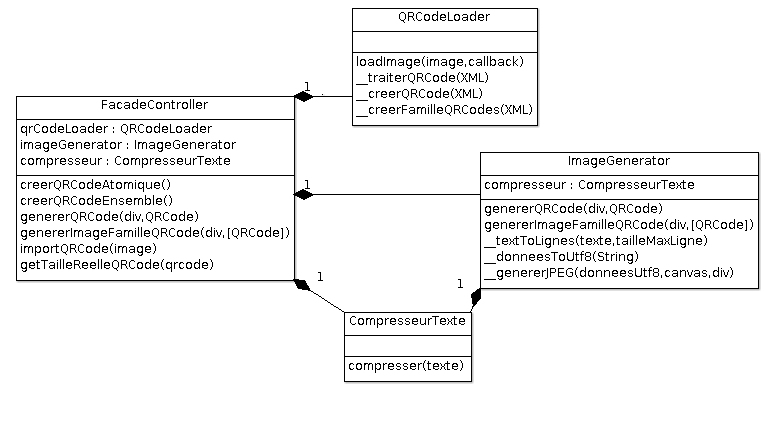
\includegraphics[scale=0.4]{img/controllerUML.png}
   \caption{Diagramme UML des classes du contrôleur}
\end{figure}

\par
La vue est responsable des interactions avec l'utilisateur (voir \ref{interfaceGraphique}). Elle offre une interface permettant de charger, de créer, d'afficher et de gérer des QR Codes.
			
		
	\section{Implémentation}
		
		\subsection{Interface graphique}
			\par
L'interface graphique offre la possibilité à l'utilisateur d'interagir avec l'application.

\begin{figure}[!h]
	\centering
   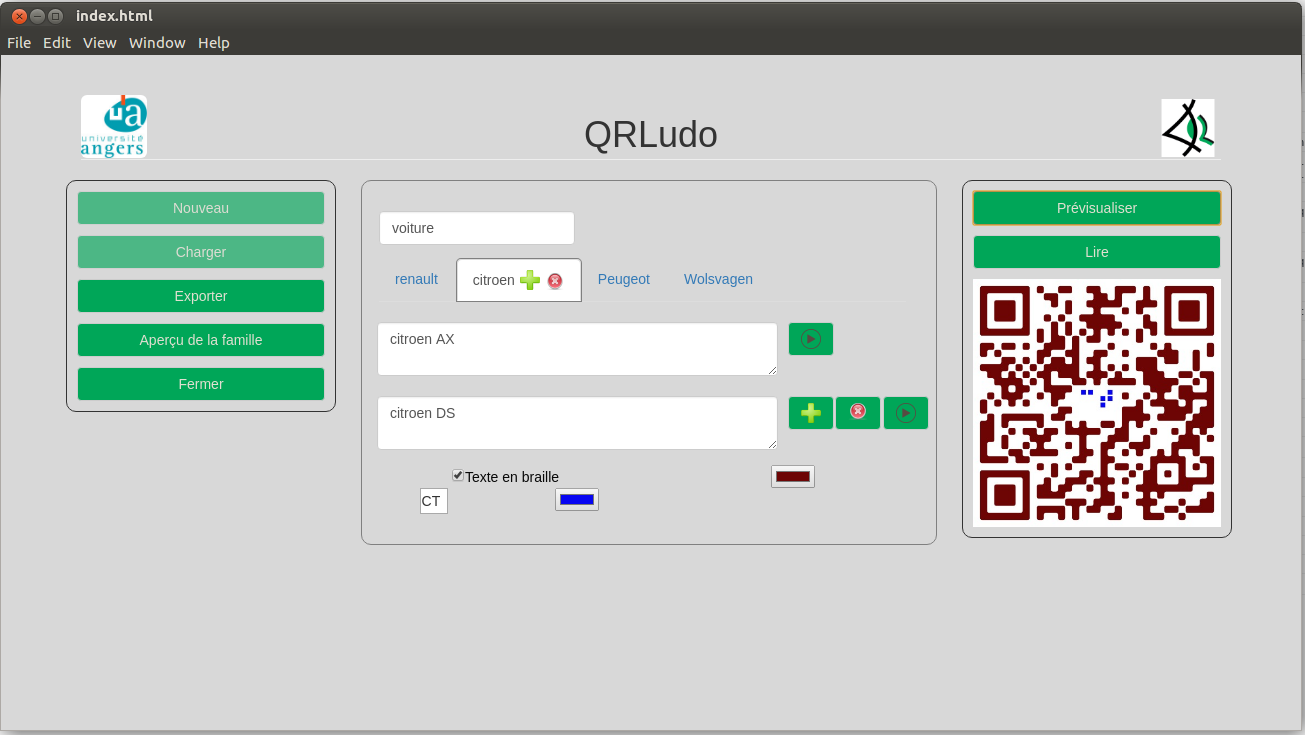
\includegraphics[scale=0.25]{img/interface.png}
   \caption{Interface de création d'une famille de qrcodes}
\end{figure}

\par
Elle constituée de trois blocs partant de la gauche vers la droite : 
\begin{enumerate}
\item Bloc 1 : partant de haut en bas, il regroupe les boutons permettant les opérations suivantes :
	\begin{itemize}
	\item la création d'un nouveau projet de QR Code unique ou d'une famille de QR Codes.
	\item le chargement ou l'importation d'un projet de QR Code unique ou d'une famille de QR Codes.
	\item l'exportation ou la sauvegarde d'un projet de QR Code unique ou d'une famille de QR Codes.
	\item l'aperçu de l'image d'une famille de QR Codes.
		\begin{figure}[!h]
			\centering
		   	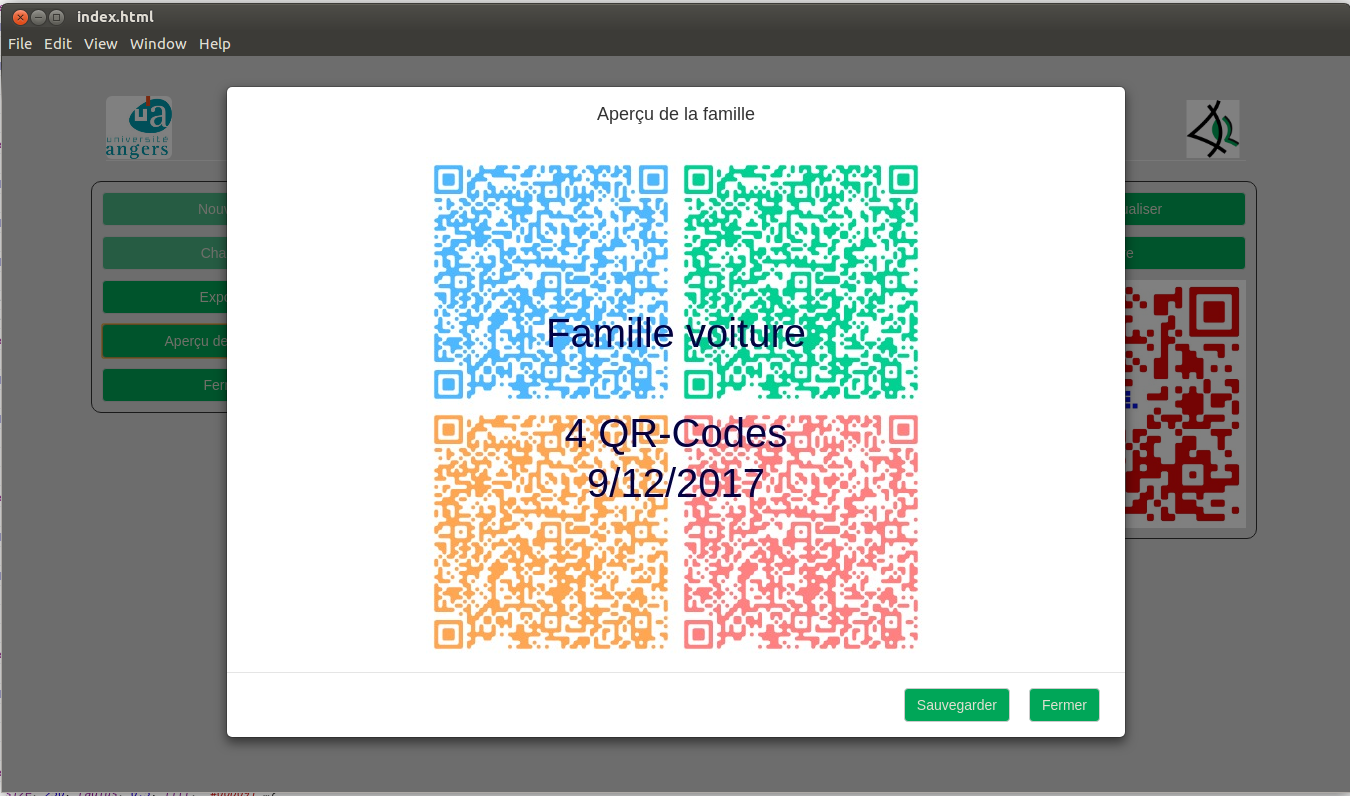
\includegraphics[scale=0.25]{img/image-famille.png}
		   	\caption{Interface de création d'une famille de qrcodes}
		\end{figure}
	
	L'image de la famille contient le nom de la famille de QR Codes, le nombre de QR Codes existant dans cette famille et la date de création du projet.\\
	Les boutons Sauvegarder et Fermer permettent respectivement de sauvegarder le projet, de fermer l'aperçu.\\
	À noter que les quatres QR Codes figurant sur l'image de la famille, ne sont que des images statiques; elles ne représentent pas des QR Codes en tant que tels.
	
	\item la fermeture d'un projet.
	\end{itemize}
	
\item Bloc 2 : il contient un formulaire qui regroupe des champs (musique ou texte). À coté de chaque champ se trouvent des boutons pour créer, supprimer et lire le contenu du champ par synthèse vocale.\\
À la fin du formulaire, de la gauche vers la droite, se trouvent :
	\begin{itemize}
	\item une case à cocher pour afficher ou masquer les options du texte en braille à savoir le texte et la couleur du texte grâce à une palette de couleur
	\item une palette de couleur pour la couleur du QR Code.
	\end{itemize}
Dans le cas d'un projet de famille de QR Codes, on note l'apparition :
	\begin{itemize}
	\item d'une zone de texte pour le nom de la famille, en haut du formulaire.
	\item d'une liste d'onglets, chacun faisant référence à un formulaire. À coté de chaque onglet, figurent deux boutons pour ajouter un onglet ou supprimer celui actif; chaque onglet représente un QR Code.
	\end{itemize}
	
\item Bloc 3 : partant du haut vers le bas, il contient : 
	\begin{itemize}
	\item un bouton pour prévisualiser un QR Code à partir des informations du formulaire (celui de l'onglet actif dans le cas d'un projet de famille de QR Codes).
	\item un bouton lire pour lire par synthèse vocale tous les champs du formulaire (le formulaire de l'onglet actif dans le cas d'un projet de famille de QR codes.
	\end{itemize}
Dans le cas d'un projet de famille de QR Code, on note l'apparition :
	\begin{itemize}
	\item d'une zone de texte pour le nom de la famille, en haut du formulaire.
	\item d'une liste d'onglets, chacun faisant référence à un formulaire. À coté de chaque onglet, figurent deux boutons pour ajouter un onglet ou supprimer celui actif; chaque onglet représente un QR Code.
		\item d'une image représentant le QR Code généré après la prévisualisation; éventuellement il y a au milieu de celle-ci un code en braille représentant le texte en braille.
	\end{itemize}
\end{enumerate}

			
		\subsection{Prévisualisation}
			\par
La prévisualisation permet de générer le QR Code avec les informations du formulaire de l'interface.\\
Nous faisons alors appel au contrôleur pour générer le QR Code (voir \ref{generation)}.
L'image générée sera celle qui sera enregistrée lors de la sauvegarde d'un projet de QR Code. Cette sauvegarde se fait de manière interactive.\\
Dans le cas d'un projet de famille de QR Code, l'interaction concerne la sauvegarde de l'image de la famille; la sauvegarde des images des QR Codes de la famille se fait de manière non interactive (automatiquement).

			
		\subsection{Génération de QR Codes}
			\par
Notre application utilise le script jquery-qrcode\footnote{https://larsjung.de/jquery-qrcode/} pour générer les images des QR Codes. Il a l'avantage d'être très souple d'utilisation et de pouvoir générer des QR Codes aux formats assez complexes. Il permet notamment d'insérer une image ou un champ texte au QR Code, ainsi que de définir les couleurs du texte central et du QR Code. Nous avons tiré profit de ces caractéristiques pour laisser la possibilité aux transcripteurs de l'institut d'insérer un texte en braille central, d'une couleur pouvant être imprimée en relief (LIEN INTRO/OBJECTIFS). Un QR Code de type atomique (REF TYPES QR) possédant des caractères centraux en braille est visible ci-dessous.\\

\begin{figure}[]
	\centering
   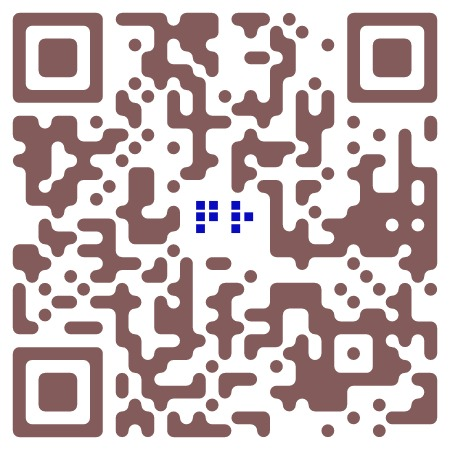
\includegraphics[scale=0.25]{img/qrsimple.jpeg}
   \caption{QR Code simple}
\end{figure}

\par
La génération des images est effectuée par la classe du Contrôleur \classe{ImageGenerator} (LIEN ARCHITECTURE). En plus des QR Codes simples, elle permet de générer des images de sauvegarde des familles de QR Codes (LIEN TYPES QR et LIEN CHARGEMENT QR). Ces images contiennent le contenu des QR Codes de la famille dans les métadonnées, et des informations sur la famille imprimées sur l'image. Un exemple d'une image famille générée par l'application est visible ci-dessous.

\begin{figure}[]
	\centering
   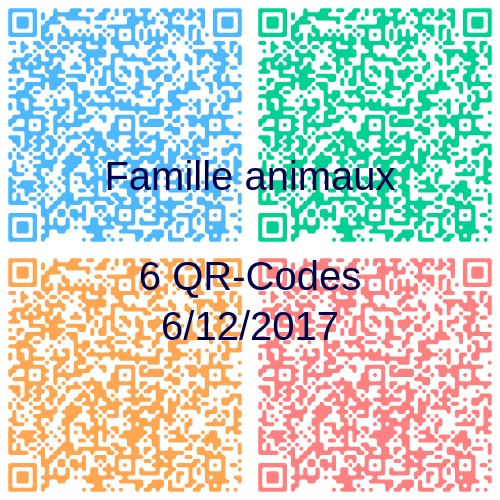
\includegraphics[scale=0.2]{img/animaux.jpeg}
   \caption{Image de sauvegarde famille}
\end{figure}
			
		\subsection{Gestion des métadonnées}
			\par
Dans l'objectif de minimiser la quantité de données stockées dans le QR Code, toutes les données qui ne sont pas nécessaires à l'application Android mais qui ont leur intérêt dans le chargement de QR Codes déjà enregistrés par l'application de bureau sont stockées dans les métadonnées de l'image du QR Code (REF Représentation des données). De plus, les images de type sauvegarde de famille (REF chargement QRCode) contiennent l'intégralité de la représentation XML des QR Codes la formant dans les métadonnées.\\
\par
Pour insérer des métadonnées dans les images générées, nous utilisons le module Node.js piexifjs\footnote{https://github.com/hMatoba/piexifjs} dans le processus suivant. Le QR Code est d'abord généré dans un canvas HTML 5, à partir duquel on va générer une image JPEG contenant dans les métadonnées le noeud racine de notre structure XML. Elles sont stockées dans le noeud XMLPacket des métadonnées EXIF\footnote{Exchangeable Image File Format}. Nous avons choisi ce noeud pour éviter la perte d'information des caractères spécifiques au français, car il peut contenir des données binaires et pas seulement des caractères ASCII comme la plupart des noeuds EXIF. Les métadonnées EXIF n'existent pas dans les fichiers PNG, et nous n'avons pas trouvé de bibliothèque permettant d'insérer un autre type de métadonnées, c'est la raison pour laquelle nous générons des images en JPG.
			
		\subsection{Chargement de QR Codes}
			\par
Dans le but de créer une application utilisable de façon concrète et régulière, nous avons créé des mécanismes permettant de modifier des QR Codes déjà enregistrés. Pour les QR Codes n'étant pas liés à d'autres (n'appartenant pas à une famille), il suffit d'enregistrer l'image représentant le QR Code en insérant dans les métadonnées le nœud racine de notre structure XML (REF REPRESENTATION DONNEES). L'utilisation du nœud XML \noeud{metadonnees} est par ailleurs trompeuse car l'intégralité de la structure XML est stockée dans les métadonnées de l'image. Nous avons choisi de procéder ainsi car nous n'avons pas trouvé de librairie Javascript permettant de scanner facilement un QR Code à partir d'un fichier image, et la quantité de données insérées dans les métadonnées de l'image est négligeable par rapport à la taille des données représentant l'image.\\
\par
Nous avons élaboré un mécanisme plus complexe en ce qui concerne l'enregistrement de QR Codes appartenant à une même famille. En effet, nous souhaitions toujours pouvoir enregistrer ces QR Codes séparément afin qu'ils puissent être imprimés, mais nous voulions empêcher la modification de l'un des QR Codes appartenant à une famille sans mettre à jour tous les autres. Pour cela, nous avons élaboré une façon d'enregistrer tous les QR Codes d'une famille dans un fichier unique, en plus des images représentant chacun des QR Codes. Nous avons choisi d'enregistrer ce fichier comme une image (REF GENERATION) contenant la représentation XML de tous les QR Codes de la famille dans ses métadonnées, et affichant certaines informations concernant la famille sous forme de texte imprimé sur l'image. Les informations imprimées sont le nom de la famille, le nombre de QR Codes contenus et la date de création. Cette image possède en outre un fond contenant quatre QR Codes colorés afin de notifier son importance et d'éviter qu'elle soit supprimée par mégarde. Pour s'assurer que cette image soit utilisée, nous avons empêché le chargement de QR Codes seuls appartenant à une famille.\\
\par
Le chargement d'un QR Code ou d'une famille de QR Codes s'effectue dans la classe \classe{QRCodeLoader} du Contrôleur. Elle instancie des sous-classes de \classe{QRCode} à partir de la racine XML des QR Codes lus dans les métadonnées de l'image, et les renvoie sous forme d'objet unique pour les QR Codes seuls ou sous forme de tableau pour les QR Codes appartenant à une famille.
			
		\subsection{Compression}
			\par
Nous avons choisi au début du projet d'utiliser une structure XML pour représenter les données stockées dans le QR Code (voir \ref{representationDonnees}). Ce choix était motivé principalement par la facilité de gestion du XML en Javascript.
\par
Le XML a toutefois posé des problèmes au niveau de la concision des QR Codes générés. Nous avons tenté de remplacer la structure XML par une structure JSON plus concise lors de la première semaine de décembre, mais nous avions déjà trop de dépendances au XML. Nous avons alors tenté d'utiliser des librairies convertissant le XML déjà généré en JSON avant l'insertion des données dans le QR Code, mais nous n'en avons trouvé aucune suffisamment fiable (les attributs des noeuds XML étaient très mal gérés, et les noeuds de même nom étaient fusionnés sans respecter leur ordre).\\
\par
Nous nous sommes donc orientés vers une solution de compression pour compenser l'intérêt qu'avait le JSON sur le XML. La solution que nous avons adoptée consiste à remplacer toutes les chaînes de caractères connues constituant le XML par un caractère UTF-8\footnote{UTF-8 (abréviation de l’anglais Universal Character Set Transformation Format - 8 bits) est un codage de caractères informatiques conçu pour coder l’ensemble des caractères du « répertoire universel de caractères codés » (Wikipédia)} prédéfini. Notre choix s'est porté sur les caractères de l'alphabet cyrillique car la probabilité qu'ils soient utilisés par les utilisateurs de l'application est très faible, et ils ne sont codés que sur deux octets (les caractères de l'UTF-8 sont représentés sur un nombre d'octets variant de un à quatre). Nous avons donc fait l'inventaire de toutes les chaînes de caractères de longueur supérieure à deux apparaissant dans notre représentation XML, et nous avons attribué à chacune un caractère de l'alphabet cyrillique. La classe \classe{CompresseurTexte} du Contrôleur se charge de remplacer par le caractère correspondant toutes les chaînes de caractères appartenant à la représentation d'un QR Code avant qu'il ne soit généré.\\
\par
Nous avons rendu cette solution la plus évolutive possible, en ajoutant deux caractères prédéfinis au début de la chaîne compressée pour notifier qu'elle a été compressée, et donc laisser la possibilité à l'application mobile avec un test simple d'interpréter les QR Codes n'ayant pas subi la compression. Le premier caractère inséré est le premier caractère de l'alphabet cyrillique, et le second est le chiffre 1, indiquant qu'il s'agit de la première version de cette méthode de compression. D'autres versions de la compression pourront ainsi être proposées dans le futur si la structure XML de représentation des données est modifiée.\\
\par
Le principal inconvénient de cette solution est qu'elle ne compresse que la représentation des données et pas les données elles-mêmes. Un QR Code contenant beaucoup de texte sera toujours volumineux. Elle est toutefois très efficace pour les QR Codes contenant peu de données comme en témoigne l'exemple ci-dessous.

\begin{figure}[!h]
\begin{adjustbox}{minipage=\textwidth,bgcolor={RGB}{240 240 240}}

\lstset{language=XML}

\begin{lstlisting}
<donneesutilisateur xmlns="http://www.w3.org/1999/xhtml" type="atomique">
  <contenu>
    <texte>Le lion appartient a la famille des felides</texte>
  </contenu>
  <famille nom="animaux" ordre="3"></famille>
</donneesutilisateur>

\end{lstlisting}

\end{adjustbox}
\caption{Données stockées dans un QR Code simple sans compression (214 octets)}

\end{figure}\textbf{}


\begin{figure}[!h]
	\centering
   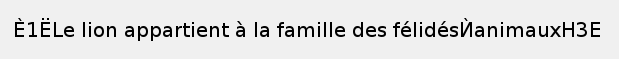
\includegraphics[scale=0.6]{img/compression.png}
   \caption{Données stockées dans un QR Code simple avec compression (63 octets, soit un gain de 70\%)}
\end{figure}
			
		\subsection{Lecture des fichiers du drive}
			\par
Pour accéder aux fichiers du drive, nous utilisons l'API\footnote{Application Programming Interface = Interface de Programmation Applicative} Google Drive REST.\\
Le paramétrage\footnote{https://developers.google.com/drive/v3/web/quickstart/nodejs} de cet API nécessite un compte Google, les modules googleapis et google-auth-library de Node.js. À l'issue du paramétrage, un dossier caché nommé .credentials est créé; ce dossier contient un fichier contenant toutes les informations privées permettant à l'application de se connecter au drive; ces informations sont chargées à chaque requête de connexion.
			
		\subsection{Limite de la taille des QR Codes}
			\par
La taille du QR Code peut influer sur sa lecture. En effet si la taille du QR Code est trop grande, l'application mobile ne pourra pas le détecter. Pour pallier ce problème, nous avons mis en place une restriction sur la taille. Pour ce faire, à chaque fois qu'il y a une requête pour une prévisualisation, on vérifie si la taille du QR Code après compression (voir \ref{compression}) ne dépasse pas un seuil que nous avons établi.\\


\chapter{Application mobile}

	\section{Application existante}
		
\par
Plusieurs fonctionnalités étaient déjà implémentées dans l'application mobile initiale (voir \ref{contexte}). Elle était notamment déjà capable de lire le contenu d'un QR Code via la synthèse vocale de l'API Google text-to-speech et d'interpréter des données structurées en JSON\footnote{JavaScript Object Notation (https://www.json.org)}. En outre, elle offrait déjà la possibilité de lire à la suite plusieurs QR Codes détectés simultanément.

\par
Notre intervention sur l'application a donc consisté à l'adapter aux nouveaux besoins.
Nous avons ainsi modifié certaines parties du code de l’application, notamment ce qui concerne l'interprétation de la structure de données qui est maintenant représentée en XML (voir \ref{representationDonnees} et \ref{compression}).\\

\par
La lecture d’un QR Code se fait donc désormais de la manière suivante. Pour les QR Codes n'appartenant pas à une famille, seul le premier champ est lu (avec la synthèse vocale s'il s'agit d'un texte, ou joué s'il s'agit d'un fichier audio). Il faut effectuer un balayage de l'écran vers la gauche ou la droite pour lire les champs adjacents.
\par
Pour les QR Codes lus simultanément et appartenant à une famille, ils sont lus dans l'ordre spécifié par la famille, tout en permettant toujours le balayage de l'écran pour passer d'un champ à un autre, ou d'un QR Code de la famille à un autre.


		
	\section{Connexion à Google Drive}
		\par
Le téléchargement des fichiers audio s'effectue en utilisant la classe \classe{DownloadManager} d'Android, qui permet de récupérer un fichier distant à partir de son URL\footnote{Uniform Resource Locator (Wikipédia)}. Elle requiert cependant des permissions pour pouvoir stocker les données téléchargées dans l'espace mémoire du téléphone. Seul l'identifiant Google Drive du fichier est stocké dans le QR Code. L'application doit donc recréer l'URL de téléchargement	à partir de cet identifiant. Une fois le fichier téléchargé, il est joué avec la classe \classe{MediaPlayer} d'Android.\\

\par
Une version antérieure de l'application utilisait l'API Google Drive REST pour télécharger les fichiers. Cette version avait pour inconvénient majeur qu'elle forçait la connexion à un compte Google pour télécharger les fichiers, ce qui était peu commode pour les utilisateurs, mais surtout qui posait de graves problème de sécurité pour le compte utilisé. En effet, tous les utilisateurs de l'application obtenaient un accès aux identifiants du compte Google utilisé.

	\section{Adaptation aux nouveaux QR Codes}
		Afin de pouvoir interpréter correctement les QR Codes scannés, nous avons créé un modèle en Java pour l'application Android. Ces classes sont calquées sur les classes du modèle de l'application de bureau (voir \ref{architecture}). Les objets du modèle sont ainsi instanciés à partir des informations lues dans les QR Codes. Ces objets sont ensuite traités pour obtenir le comportement voulu selon chaque type de QR Code scanné.

\chapter{Conclusion}
	\par
Tout au long du développement, nous nous sommes efforcés de produire des applications répondant concrètement aux demandes de l'institut Montéclair, tout en gardant à l'esprit que les besoins de l'institut pourraient évoluer. Par conséquent, nos applications ne se veulent pas des versions définitives. En dehors du travail qui reste à effectuer pour les rendre totalement utilisables au quotidien, nous avons tenté de les rendre ouvertes à l'extension pour des versions futures avec peut-être d'autres types de QR Codes, d'autres types de contenus ou d'autres méthodes d'optimisation de la quantité de données contenues dans les QR Codes.\\
Cette volonté s'est traduite par la réalisation d'une architecture des classes souple et non spécifique aux besoins qui nous ont été transmis. Nous avons en outre fait en sorte que la compression des données, qui est la partie la plus susceptible d'être modifiée, soit modulable tout en restant facilement compatible avec les QR Codes que nous générons actuellement.\\

\par
Il reste toutefois une dernière phase de développement avant de pouvoir livrer un couple d'applications totalement fonctionnelles. Les modifications restantes concernent principalement l'interface graphique de l'application de bureau, afin qu'elle soit plus ergonomique avec un système de liste de QR Codes plutôt que d'onglets, un système de glisser-déposer de fichiers provenant de Google Drive, et l'implémentation de la création de QR Codes de type ensemble, permettant de télécharger un ensemble de fichiers audio sans les jouer.
\par
Elles concernent également la complétion de l'interprétation des QR Codes par l'application mobile, afin de gérer dynamiquement le téléchargement de fichiers à la lecture, et l'ajout de messages vocaux à destination de l'utilisateur.\\

\par
Lorsque cette phase de finalisation sera terminée, un nouveau projet pourra débuter à partir de là où nous l'avons laissé, comme nous l'avons fait à partir de l'application mobile initiale. En plus de l'implémentation d'éventuelles nouvelles demandes de l'institut Montéclair, un travail complexe mais intéressant pourra être effectué pour compresser le contenu des QR Codes de manière plus efficace, en compressant le texte contenu dans les QR Codes à partir d'un dictionnaire fixe externe. Une solution de transformation du texte en son directement sur l'application de bureau pourrait également permettre de créer des QR Codes contenant des textes de grande taille.



\addappheadtotoc
\appendixpage

\appendix

\section{Organisation}

	\subsection{Répartition des tâches}
\subsection{Calendrier}

		
		
\section{Manuel Utilisateur}

	\input{Annexes/manuel.tex} 


\end{document}